\documentclass[10pt,twocolumn]{article}
\usepackage[10pt,nocopyright,inchmargins]{sigmin}
\usepackage[letterpaper, breaklinks, pdfborder={0 0 0}]{hyperref}
\usepackage[square,comma,numbers,sort&compress]{natbib}
\usepackage{times}
\usepackage{microtype}
\usepackage{booktabs}
\usepackage{mathptmx}
\usepackage{graphicx}
\usepackage{url}
\usepackage{listings}
\usepackage{hyperref}
\usepackage{underscore}
\usepackage[T1]{fontenc}
\usepackage{amsmath}
\usepackage{amsfonts}
\usepackage{amssymb}
\usepackage{verbatim}
\usepackage{color}
\usepackage{xspace}
\usepackage{multirow}
\usepackage{relsize}
\usepackage{fancyvrb}
\usepackage{pgfplots}
\lstset{language=C}          % Set your language (you can change the language for each code-block optionally)

\pgfplotsset{width=7.3cm,compat=1.8}
\usepgfplotslibrary{statistics}
\usepgfplotslibrary{units}
\makeatletter
\pgfplotsset{
    boxplot/hide outliers/.code={
        \def\pgfplotsplothandlerboxplot@outlier{}%
    }
}
\makeatother
\renewcommand{\ttdefault}{pxtt}   %% better \tt font

%% Ensure ligatures (e.g., ``fine official flag'') can be copy/pasted from PDF.
\input{glyphtounicode}
\pdfgentounicode=1

\widowpenalty=5000
\clubpenalty=5000

\newif\ifdraft\drafttrue
\newif\ifnotes\notestrue
\ifdraft\else\notesfalse\fi

% Define \XXX, \XXX[notes] and \XXX[author][notes]
\definecolor{xxxcolor}{rgb}{0.8,0,0}
\makeatletter
\long\def\XXX{\@ifnextchar[{\@XXX}{\@XXX[]}}
\long\def\@XXX[#1]{\@ifnextchar[{\@@@XXX{#1}}{\@@XXX{#1}}}
\ifnotes
% Show XXX comments
\long\def\@@XXX#1{{\color{xxxcolor} XXX #1}\xspace}
\long\def\@@@XXX#1[#2]{{\color{xxxcolor} XXX (#1) #2}\xspace}
\else
% Hide XXX comments
\long\def\@@XXX#1{\ignorespaces}
\long\def\@@@XXX#1[#2]{\ignorespaces}
\fi
\makeatother


\input{code/fmt}

\begin{document}
\begin{figure}
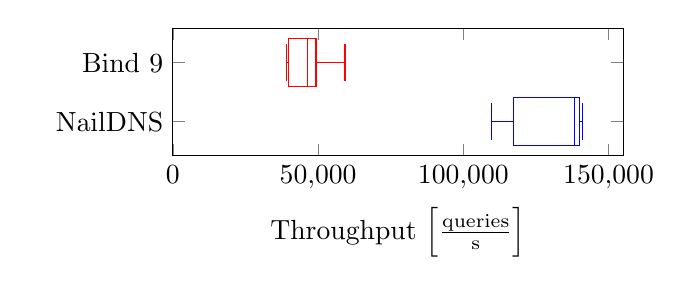
\begin{tikzpicture}
\begin{axis}[
  y=0.75cm,
  ytick={1,2},
  yticklabels={NailDNS, Bind 9},
  xmin=0,
  xlabel ={Throughput},
  x unit ={\frac{\text{queries}}{s}},
  scaled x ticks = false,
  x tick label style = {/pgf/number format/fixed}
]
\addplot+[boxplot]
  table[row sep=\\,y index=0] {
data\\
 140950.177719\\
 137100.337896\\
 140575.256869\\
 139215.019250\\
 109667.926913\\
 125123.464186\\
 139507.888042\\
 };
\addplot+[boxplot]
  table[row sep=\\,y index=0] {
data\\
50713.068173\\
45230.492090\\
47824.395302\\
39167.055247\\
47234.594953\\
59239.056531\\
40436.939492\\
 };
\end{axis}
\end{tikzpicture}

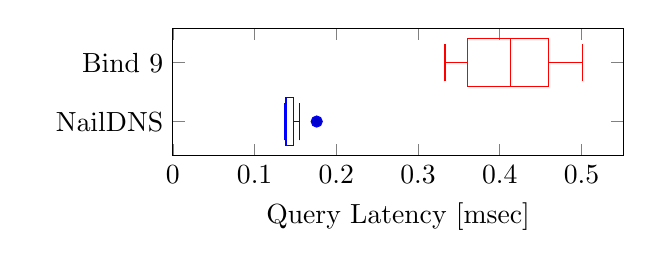
\begin{tikzpicture}
\begin{axis}[
  y=0.75cm,
  ytick={1,2},
  yticklabels={NailDNS, Bind 9},
  xmin=0,
  xlabel ={Query Latency},
  x unit= {msec},
  scaled x ticks = false
]
\addplot+[boxplot]
  table[row sep=\\,y index=0] {
data\\
0.137\\
0.141\\
0.138\\
0.139\\
0.176\\
0.155\\
0.139\\
 };
\addplot+[boxplot]
  table[row sep=\\,y index=0] {
data\\
0.388\\
0.434\\
0.411\\
0.501\\
0.416\\
0.333\\
0.486\\
 };
\end{axis}
\end{tikzpicture}

\caption{A box plot comparing the performance of the Nail-based DNS server compared to
  BIND 9.5.5 on 50,000 domains.  The boxes show the interquartile range, with the middle showing the
  median result. The dots show outliers.}
\label{fig:perf-dns}

\end{figure}

\end{document}